\section[Basics]{Grundlagen}

\begin{frame}[c]{}
  \begin{center}
    \structure{\Large \insertsection}
  \end{center}
\end{frame}

\begin{frame}{Digital Native}
  \begin{columns}[T]
  \column{100pt}
    Was heißt das?\\
    \vspace{0.5cm}
    \uncover<2->{aufgewachsen mit\\}
    \begin{itemize}
      \item<3->... Computern
      \item<9->... einem Handy
      \item<13->... Konsolen
      \item<17->... Diensten
    \end{itemize}
    \vspace{0.5cm}
    \uncover<30->{Was brauchen wir?\\}
    \begin{itemize}
      \item<31->... Internet
      \item<32->... Benutzername
      \item<32->... Passwort
    \end{itemize}

    
  \column{179pt}
    \includegraphics<3>[height=7cm]{digitalnatives/computer1.jpg}
    \includegraphics<4>[height=7cm]{digitalnatives/computer2.jpg}
    \includegraphics<5>[height=7cm]{digitalnatives/computer3.jpg}       
    \includegraphics<6>[height=7cm]{digitalnatives/computer4.jpg}       
    \includegraphics<7>[height=7cm]{digitalnatives/computer5.jpg}       

    \includegraphics<9>[height=7cm]{digitalnatives/mobile1.jpg}
    \includegraphics<10>[height=7cm]{digitalnatives/mobile2.jpg}
    \includegraphics<11>[height=7cm]{digitalnatives/mobile3.jpg}       

    \includegraphics<13>[height=7cm]{digitalnatives/console1.jpg}
    \includegraphics<14>[height=7cm]{digitalnatives/console2.jpg}
    \includegraphics<15>[height=7cm]{digitalnatives/console3.jpg}
    
    \includegraphics<18>[height=7cm]{digitalnatives/services0.jpg}
    \includegraphics<19>[height=7cm]{digitalnatives/services1.jpg}
    \includegraphics<20>[height=7cm]{digitalnatives/services2.jpg}
    \includegraphics<21>[height=7cm]{digitalnatives/services3.jpg}
    \includegraphics<22>[height=7cm]{digitalnatives/services4.jpg}
    \includegraphics<23>[height=7cm]{digitalnatives/services5.jpg}
    \includegraphics<24>[height=7cm]{digitalnatives/services6.jpg}
    \includegraphics<25>[height=7cm]{digitalnatives/services7.jpg}
    \includegraphics<26>[height=7cm]{digitalnatives/services8.jpg}
    \includegraphics<27>[height=7cm]{digitalnatives/services9.jpg}
    \includegraphics<28>[height=7cm]{digitalnatives/services10.jpg}
    \includegraphics<29>[height=7cm]{digitalnatives/services11.jpg}

    \includegraphics<31>[height=7cm]{digitalnatives/online.jpg}

    \includegraphics<32>[height=7cm]{digitalnatives/online2.jpg}
    
  \end{columns}
\end{frame}

\section[Passwörter]{Passwörter}

\begin{frame}{Benutzername/Passwort} 
  \begin{itemize}
    \item ein Schlüssel
    \item<2-> WER ich bin
    \item<2-> dass ich es TATSÄCHLICH bin
    \item<3-> zur Identifikation
    \begin{itemize}
      \item<4-> ``ich bin'': Aussehen, Fingerabdruck
      \item<5-> ``ich habe'': Schlüssel, Keycard, Mitgliedsausweis
      \item<6->\alert<8>{``ich weiß''}: geheimes Handzeichen, Klopfzeichen\uncover<8->{, \alert<8>{Passwort}}
    \end{itemize}
    \item<7-> Benutzername und Passwort?
    \item<9-> \alert{Problem:} Der andere muss mein Passwort auch wissen!
  \end{itemize}
\end{frame}

\begin{frame}{Passwörter speichern} 
  Nicht meine Verantwortung, aber mein Schaden!
  \begin{itemize}
    \item<2-> \only<2>{Klartext, unverschlüsselt}\only<3->{\xout{Klartext, unverschlüsselt}}: \hfill{\tiny{\texttt{meinPasswort}}}
    \item<4-> \only<4-5>{verschlüsselt, entschlüsselbar}\only<6->{\sout{verschlüsselt, entschlüsselbar}}: \uncover<5->{\hfill{\tiny{\texttt{trowssaPniem}}}}
    \item<7-> 1-Weg-verschlüsselt, ``gehasht'': \uncover<8->{\hfill{\tiny{\texttt{6993468f79db35810a3ce10a602be8d7}}}}\\
    \begin{itemize}
      \item<9->nicht umkehrbar
      \item<9->gleiches Passwort liefert immer gleichen Hashwert
      \item<10->eingegebenes Passwort verschlüsseln und Ergebnisse vergleichen
    \end{itemize}
    \item<11->Ist mein Passwort dadurch sicher?
  \end{itemize}
\end{frame}


\begin{frame}[c]{Hashcracking}
  \only<1>{
    \begin{center}
      \structure{\Large Live DEMO}
    \end{center}
  }

  \only<2->{
    \begin{center}
      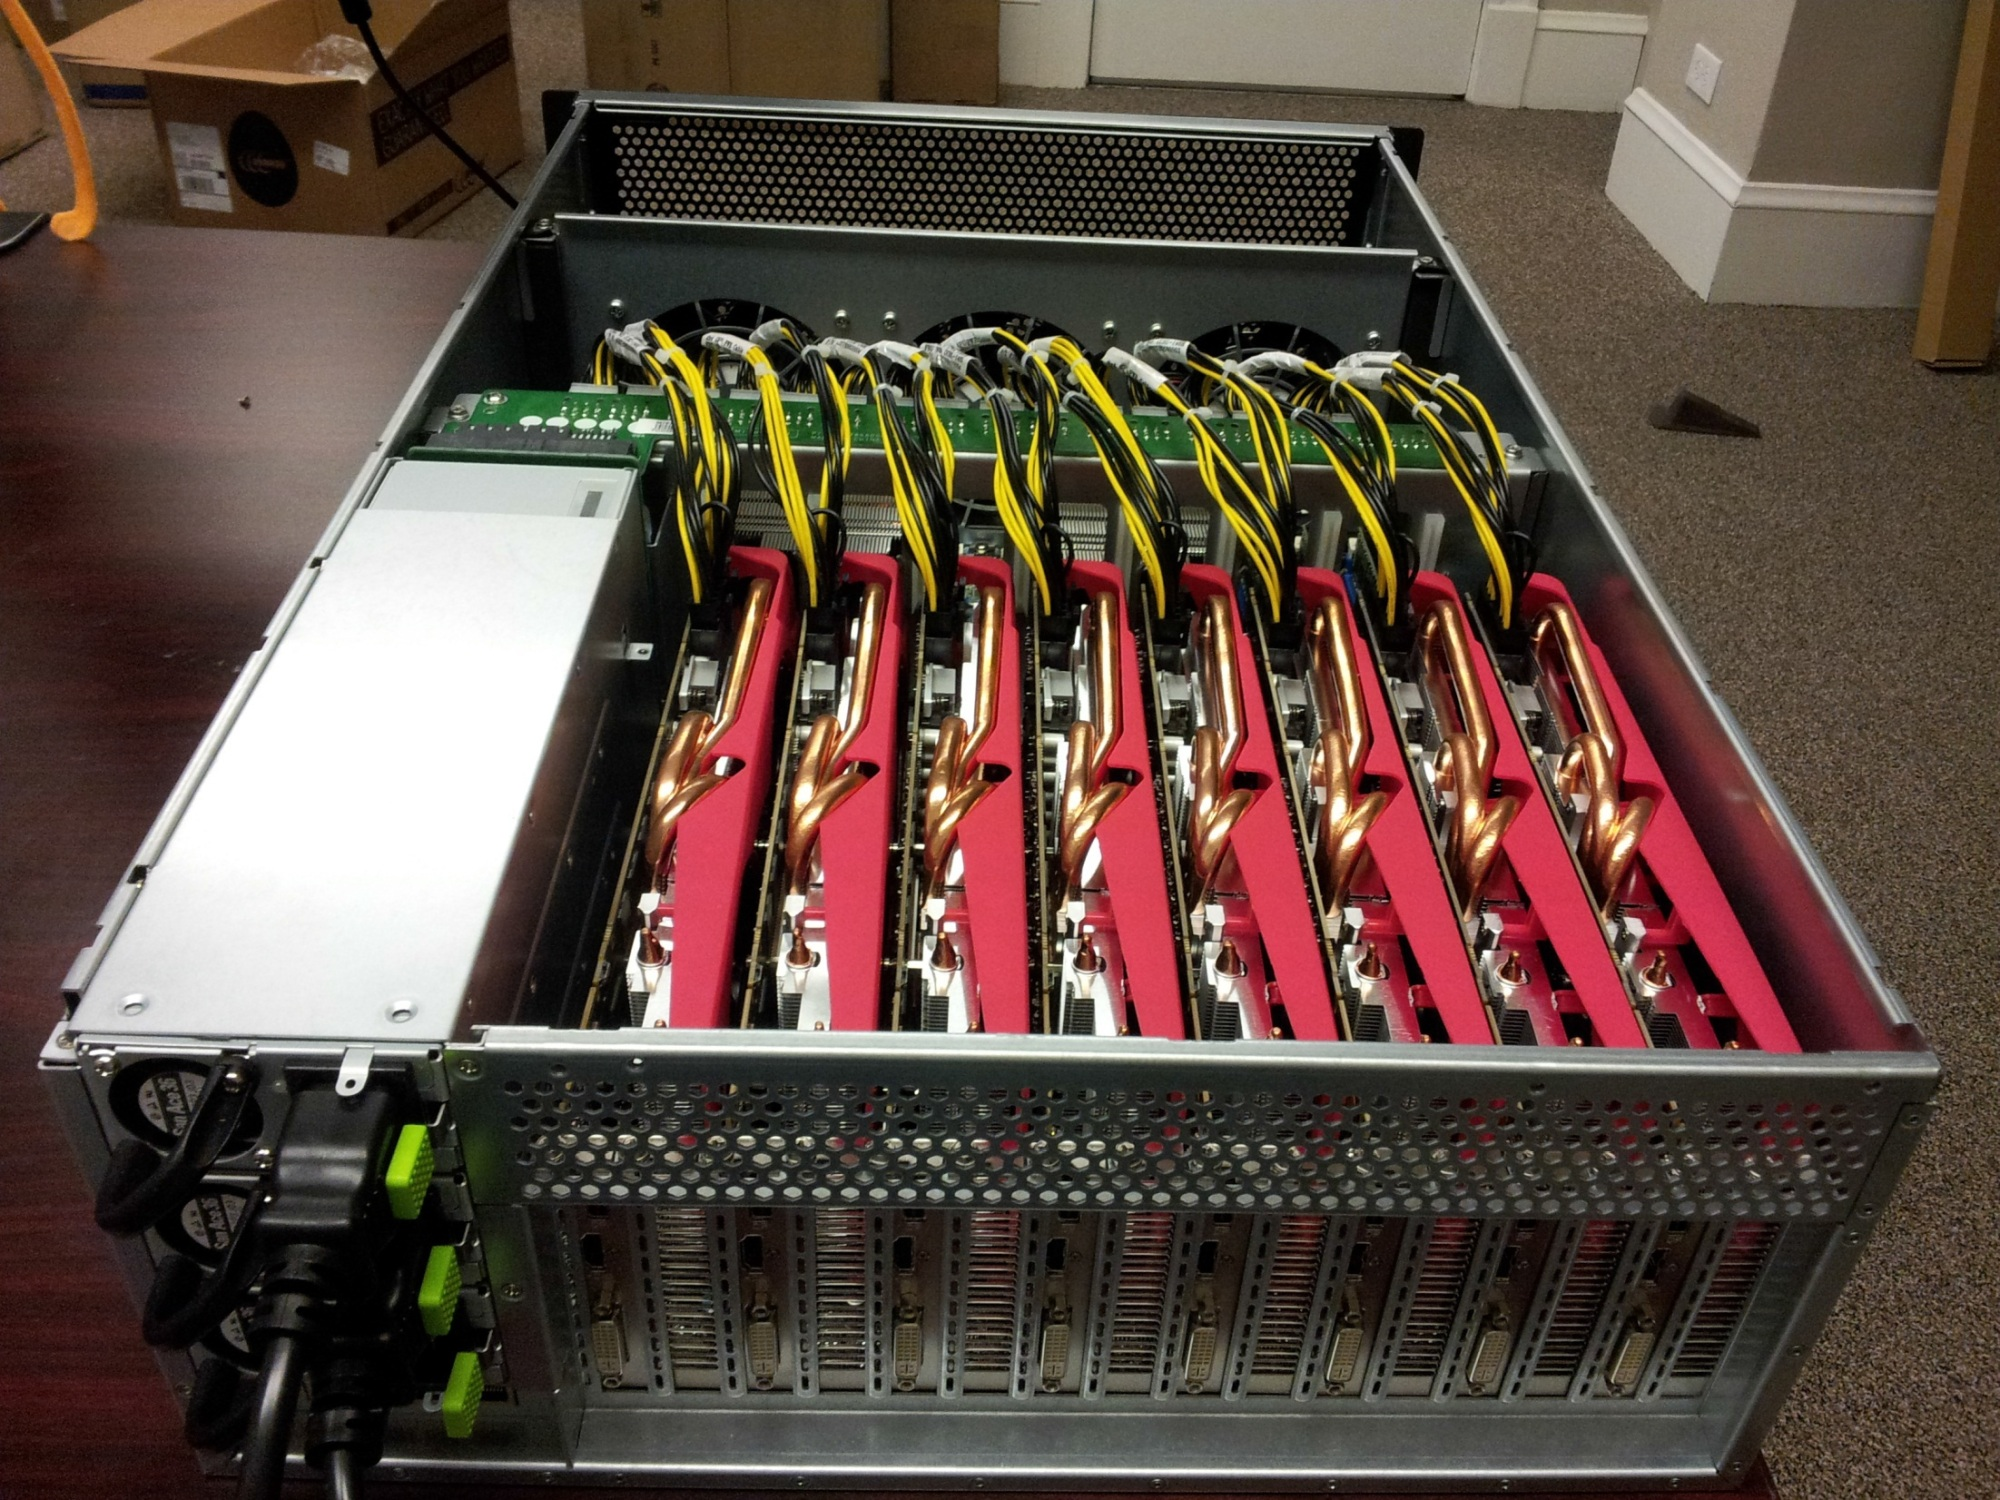
\includegraphics[height=5cm]{digitalnatives/hashcat-cluster.jpg}
    \end{center}
    \begin{itemize}
      \item 348 Milliarden Windows Passwörter pro Sekunde
      \item 8 Zeichen Windows7/8 Passwort: 5,5 Stunden
      \item 14 Zeichen WinXP Passwort: 6 Minuten
    \end{itemize}

  }

\end{frame}

\begin{frame}{Was Hacker also machen ...}
  \begin{itemize}
    \item<1-> besorge Passwörter, Benutzernamen und E-Mail von Service X
    \item<2-> knacke Passwörter
    \item<3-> probiere andere Dienste!
    \item<4-> vor allem E-Mail!
  \end{itemize}
  \uncover<5->{
    geknackte Dienste:
    \tiny{
    \begin{itemize}
      \item Microsoft: Online-Store (Klartext!)
      \item Twitter: 250.000 Datensätze
      \item Phillips: 200.000 Datensätze
      \item Battle.net (Blizzard)
      \item Gamigo: 11 Mio. Passwörter
      \item NVidia Forum: 400.000 Datensätze
      \item Yahoo!: 400.000 Datensätze (Klartext!)
      \item Last.fm: 2,5 Mio. Passwörter
      \item LinkedIn: 6,5 Mio. Passwörter
      \item Foren, Dating-, Spieleplattformen, ...
    \end{itemize}
    }
  }
\end{frame}

\begin{frame}{So ... what?}
  Was bedeutet das für mich, wenn mein Passwort geknackt ist?!
  \begin{itemize}
    \item<2-> Identitätsdiebstahl
  \end{itemize}

  \uncover<3->{
    Und wie schütze ich mich davor?
    \begin{itemize}
      \item<4-> Gar nicht! \only<5->{\alert{Außerhalb meiner Verantwortung!}}
      \item<6-> unterschiedliche Passwörter! \only<7->{\alert{Meine Verantwortung!}}
    \end{itemize}
  }
\end{frame}


\begin{frame}{Passwörter verwalten}
  \begin{enumerate}
    \item<1-> Passwort Manager
      \begin{itemize}
        \item<2-> z.B. KeePass \tiny{(gratis, für Win/Mac/Linux, IPhone, Android, Windows Phone, Browser)}
      \end{itemize}
    \item<3-> Passwörter mit System
      \begin{itemize}
        \item<4->Basis-Kennwort: \hfill{\texttt{1S:wG1Lp}}
	\item<5->Servicename: \hfill{facebook}
	\item<6->1. Buchstabe, Länge und 3. Buchstabe: \hfill{\texttt{f8c}}
	\item<7->an 3., 6. und 9. Stelle einfügen: \hfill{\texttt{1S\alert{f}:w\alert{8}G1\alert{c}Lp}}
	\item<8->Instagram: \hfill{\texttt{1Si:w9G1sLp}}
	\item<9->GMail: \hfill{\texttt{1SG:w5G1aLp}}
      \end{itemize}
    \item<10-> Lügen, Betrügen und Verfälschen!
    \item<11-> \alert{Gebt niemals eure Passwörter her!}


  \end{enumerate}

\end{frame}

